\documentclass[12pt]{article}

%%%%%% This thesis template was originally created by Zhiya Zuo and Erin Kaufman in May 2019, and revised by Marina Zhang and Erin Kaufman in July 2022. %%%%%%

%%%%%% start: define some names here %%%%%%
\newcommand{\longvertspacing}{~\\~\\~\\~\\~\\~\\}
\newcommand{\mylinespacing}{\vspace{1em}}
\newcommand{\myoptpg}{\textbf{THIS PAGE IS OPTIONAL}}
\newcommand{\mytitle}{Machine Learning Based Reconstruction Studies For DUNE Near Detector}
\newcommand{\sourcetitle}{Poul Anderson}
\newcommand{\myname}{Orgho Neogi}
%%%% replace My Degree with Doctor of Philosophy, Doctor of Musical Arts, Master of Science, Master of Arts, or Master of Fine Arts %%%%
\newcommand{\degreetype}{\capitalize{Doctor of Philosophy}} 
\newcommand{\mydegree}{\capitalize{Doctor of Philosophy}}
\newcommand{\myprogram}{\capitalize{Physics \& Astronomy}}
%%%% choose: May, August, December  %%%%
\newcommand{\mymonth}{May}
\newcommand{\myyear}{2024}
\newcommand{\myadvisor}{Jane Nachtman}
\newcommand{\committeememberA}{Yaser Onel}
\newcommand{\committeememberB}{Milind Diwan}
\newcommand{\committeememberC}{Mary Hall Reno}
\newcommand{\committeememberD}{Committee Member Name}
%%%%%% start: define some names here %%%%%%

\usepackage{geometry}
\usepackage{float}
\usepackage{amsmath}
 \geometry{
 letterpaper,
 left=2.54cm,
 right=2.54cm,
 bottom=2.54cm,
 top=2.54cm,
 }
\usepackage[utf8]{inputenc}

%% ref related
\usepackage{varioref}
\usepackage[linktocpage=true]{hyperref}
\usepackage[capitalise,noabbrev]{cleveref}
%% toc
\usepackage{tocloft}
%%% dots: https://tex.stackexchange.com/questions/53898/how-to-get-lines-with-dots-in-the-table-of-contents-for-sections
\renewcommand{\cftsecleader}{\cftdotfill{\cftdotsep}}
\renewcommand{\cftfigleader}{\cftdotfill{\cftdotsep}}
\renewcommand{\cfttableader}{\cftdotfill{\cftdotsep}}
%%% adjust sectional unit title fonts in toc
\renewcommand{\cftsecfont}{\normalfont\MakeUppercase} 
\renewcommand{\cftsubsecfont}{\normalfont}
\renewcommand{\cftsubsubsecfont}{\normalfont}
\renewcommand{\cftsecpagefont}{\normalfont}
%%% use figure/table.num for the lot and lof
%\renewcommand{\cftfigfont}{Figure~\alph{fig}.}
%% source: https://tex.stackexchange.com/questions/419103/how-to-change-the-numbering-style-in-list-of-table-and-list-of-figures
\renewcommand{\cftfigpresnum}{Figure }
\renewcommand{\cftfigaftersnum}{.\hspace{1ex}}
\renewcommand{\cfttabpresnum}{Table }
\renewcommand{\cfttabaftersnum}{.\hspace{1ex}}
%%% increase spacing between entries in toc
\setlength{\cftparskip}{2ex}
%%% decrease spacing between number and title as well as indent
%\setlength{\cftfignumwidth}{10ex}
%\setlength{\cfttabnumwidth}{8ex}
\setlength{\cftfignumwidth}{10.5ex}
\setlength{\cfttabnumwidth}{8ex}
\setlength{\cftfigindent}{0ex}
\setlength{\cfttabindent}{0ex}
%%% title names
%%% center uppercase toc titles
%% https://tex.stackexchange.com/a/255699/154200
\renewcommand{\cfttoctitlefont}{\hspace*{\fill}\normalsize\MakeUppercase}
\renewcommand{\cftaftertoctitle}{\hspace*{\fill}}
\renewcommand{\contentsname}{table of contents}
\renewcommand{\cftlottitlefont}{\hfill\normalsize\MakeUppercase}
\renewcommand{\cftafterlottitle}{\hfill}
\renewcommand{\cftloftitlefont}{\hfill\normalsize\MakeUppercase}
\renewcommand{\cftafterloftitle}{\hfill}
%% this package binds all indices to toc
\usepackage[nottoc]{tocbibind}
%%% remove toc numbering
\makeatletter
\let\latexl@section\l@section
\def\l@section#1#2{\begingroup\let\numberline\@gobble\latexl@section{#1}{#2}\endgroup}
\let\latexl@subsection\l@subsection
\def\l@subsection#1#2{\begingroup\let\numberline\@gobble\latexl@subsection{#1}{#2}\endgroup}
\let\latexl@subsubsection\l@subsubsection
\def\l@subsubsection#1#2{\begingroup\let\numberline\@gobble\latexl@subsubsection{#1}{#2}\endgroup}
\makeatother
%% set figure path
\usepackage{graphicx}
\graphicspath{{figures/}}
%% captions
\usepackage{boxhandler}
\usepackage{caption}
\captionsetup{labelsep=period, justification=raggedright, singlelinecheck=false}
%% appendix
\usepackage{appendix}

%% uses times font
\usepackage{mathptmx}
%% set fontsize
\fontsize{12}{1} \selectfont
%% set line spacing
\usepackage{setspace}
\singlespacing
%% set par indent
%\usepackage{indentfirst}
\setlength{\parindent}{6.5ex}
%% customize heading styles
\usepackage[indentafter]{titlesec}
\usepackage[numbers]{natbib}
%%%% heading 1
\titleformat{\section}
  {\normalsize\center}
  {}
  {0pt}
  {\MakeUppercase}
%%%% heading 2
\titleformat{\subsection}
  {\normalsize\center\bf}
  {}
  {0pt}
  {\capitalize}
%%%% heading 3
\titleformat{\subsubsection}
  {\normalsize\bf}
  {}
  {0pt}
  {\capitalize}
%%%% heading 4
\titleformat{\paragraph}
  {\normalsize\bf\itshape}
  {}
  {0pt}
  {\capitalize}
%\titleformat{⟨command⟩}[⟨shape⟩]{⟨format⟩}{⟨label⟩}{⟨sep⟩}{⟨before-code⟩}[⟨after-code⟩]

%% a new center environment
\newenvironment{tightcenter}{%
  \setlength\topsep{0pt}
  \setlength\parskip{0pt}
  \begin{center}
}{%
  \end{center}
}
%% adjust quotation environment margin
\renewenvironment{quote}{%
   \list{}{%
     \leftmargin0cm   % this is the adjusting screw
     \rightmargin\leftmargin
   }
   \item\relax
}
{\endlist}

%%%%%% capitalize from stackexchange %%%%%% 
\usepackage{ifxetex}

\usepackage{xparse}

\ExplSyntaxOn
\NewDocumentCommand{\capitalize}{>{\SplitList{~}}m}
 {
  \seq_clear:N \l_capitalize_words_seq
  \ProcessList{#1}{\CapitalizeFirst}
  \seq_use:Nn \l_capitalize_words_seq { ~ }
 }
\NewDocumentCommand{\CapitalizeFirst}{m}
 {
  \capitalize_word:n { #1 }
 }

\sys_if_engine_pdftex:TF
 {
  \cs_set_eq:Nc \capitalize_tl_set:Nn { protected@edef }
 }
 {
  \cs_set_eq:NN \capitalize_tl_set:Nn \tl_set:Nn
 }

\cs_new_protected:Nn \capitalize_word:n
 {
  \capitalize_tl_set:Nn \l_capitalize_word_tl { #1 }
  \seq_if_in:NfTF \g_capitalize_exceptions_seq { \tl_to_str:n { #1 } }
   % exception word
   { \seq_put_right:Nn \l_capitalize_words_seq { #1 } } % exception word
   % to be uppercased
   { \seq_put_right:Nx \l_capitalize_words_seq { \tl_mixed_case:V \l_capitalize_word_tl } }
 }
\cs_generate_variant:Nn \tl_mixed_case:n { V }
\NewDocumentCommand{\AppendToList}{m}
 {
  \clist_map_inline:nn { #1 }
   {
    \seq_gput_right:Nx \g_capitalize_exceptions_seq { \tl_to_str:n { ##1 } }
   }
 }
\cs_generate_variant:Nn \seq_if_in:NnTF { Nf }
\seq_new:N \l_capitalize_words_seq
\seq_new:N \g_capitalize_exceptions_seq
\ExplSyntaxOff

\AppendToList{a,is,of,óf}
%%%%%% capitalize from stackexchange %%%%%% 

\title{\MakeUppercase{\normalsize\mytitle}\vspace{-2em}}
\author{\vspace{-5ex}}
\date{\vspace{-5ex}}

\begin{document}

\maketitle

%% roman for frontmatter
\pagenumbering{roman}
\thispagestyle{empty}
\longvertspacing
\begin{tightcenter}
    by
\end{tightcenter}
\mylinespacing
\begin{tightcenter}
    \myname
\end{tightcenter}
\longvertspacing
\begin{tightcenter}
A thesis submitted in partial fulfillment \\
of the requirements for the \degreetype\\
degree in \myprogram~in the  \\
Graduate College of \\
The University of Iowa
\end{tightcenter}
\mylinespacing
\begin{tightcenter}
\mymonth~\myyear
\end{tightcenter}
\mylinespacing
\begin{tightcenter}
Thesis Committee: Name of Thesis Supervisor, \myadvisor
\end{tightcenter}
\begin{tightcenter}
\committeememberA
\end{tightcenter}
\begin{tightcenter}
\committeememberB
\end{tightcenter}
\begin{tightcenter}
\committeememberC
\end{tightcenter}
%\begin{tightcenter}
%\committeememberD
%\end{tightcenter}
%% copyright page %%

%\pagenumbering{gobble} 
\vspace*{\fill} 
\begin{quote} 
\centering 
Copyright by\\ 
\mylinespacing
\myname \\
\mylinespacing
\myyear \\
\mylinespacing
All Rights Reserved \\
\mylinespacing
\myoptpg
\end{quote}
\vspace*{\fill}

%% copyright page %%

\pagenumbering{roman} 
\setcounter{page}{1}
%% dedication page %%
%\vspace*{\fill} 
\noindent
Prior to your first thesis deposit, delete this text and type your dedication here.  The entire dedication should be single spaced and centered vertically and horizontally on the page.  This text may be altered between first and final deposit.
\begin{quote}
\centering
\mylinespacing
\myoptpg
\end{quote}
\vspace*{\fill}
%% dedication page %%

%% epigraph page %%
\vspace*{\fill} 
\begin{quote}
\centering
 I have yet to see any problem, however complicated, which, when looked at in the right way did not become still more complicated.
 
\mylinespacing
\sourcetitle \\
\mylinespacing
\end{quote}
\vspace*{\fill}

%% epigraph page %%

%% ack page %%
%\begin{doublespace}
\begin{tightcenter}
ACKNOWLEDGMENTS
\mylinespacing
\end{tightcenter}

Prior to your first thesis deposit, replace this text with your acknowledgements.  This text should be double spaced and each paragraph should be indented.  

\mylinespacing
\begin{tightcenter}
\myoptpg
\end{tightcenter}
\end{doublespace}

%% ack page %%

%% abs page %%
\begin{doublespace}
\begin{tightcenter}
ABSTRACT
\mylinespacing
\end{tightcenter}

Prior to your first thesis deposit, replace this text with the text of your scientific/ scholarly abstract. The text of this abstract should be double spaced and each new paragraph should be indented. 

\mylinespacing
\mylinespacing
\begin{tightcenter}
\textbf{This abstract is required for everyone except DMA and MFA students.}
\end{tightcenter}
\end{doublespace}

%% abs page %%

%% public abs page %%
\begin{doublespace}
\begin{tightcenter}
PUBLIC ABSTRACT
\mylinespacing
\end{tightcenter}

Prior to your thesis deposit, replace this text with the text of your public abstract.  The text of this abstract should be double spaced and each new paragraph should be indented.

\textbf{This abstract is required for all thesis/dissertations.}  This abstract may be up to 250 words and should be written for a non-academic lay audience.  In writing your public abstract, avoid jargon and technical language as much as possible. 

The ability to communicate research simply and clearly is an important skill. The public abstract helps convey ideas beyond one’s immediate academic circle, facilitating communication with colleagues who do different kinds of work and possess different dimensions of training.

Think of your public abstract as your “elevator pitch” or what you might tell someone who asks, “What is your thesis about?”  You may only have a few minutes to explain it to them while keeping their attention and using terminology you are sure they will understand without further lengthy explanation.    

Another way to think of your public abstract is like the description you would read on the inside of a book cover.

\end{doublespace}

%% public abs page %%

%% content lists %%
\setcounter{tocdepth}{3} % can change 2 for heading 2
\tableofcontents
\newpage
\listoftables
\newpage
\listoffigures

%% content lists %%

%% preface %%
%\begin{doublespace}
\begin{tightcenter}
\section{PREFACE}
%%PREFACE
\mylinespacing
\end{tightcenter}

This page is OPTIONAL. The Preface should be double spaced and new paragraphs should be indented.  

\mylinespacing
\mylinespacing
\begin{tightcenter}
\myoptpg
\end{tightcenter}
\end{doublespace}
%% preface %%

%% arabic for the rest
\pagenumbering{arabic}

\begin{doublespace}
  %% main contents %%
  \section{heading 1: my chapter 1}

Heading 1 is the style you should use for the following headings in your thesis: List of Tables, List of Figures (List of Abbreviations, Schemes, and so on), Chapter titles, References, and Appendix titles. If you are writing in APA style, note that the titles formatted as Heading 1 do not count as an APA heading.  

I want to cite something here \parencite{zuo2019standing}. I want to want to try cite~\textcite{zuo2019standing} with in-line style.

\subsection{heading 2: Use for Your broadest Subheading Level, Centered, Bold, Title Case}

Heading 2 is the first major subheading style. If you are writing in APA style, this heading corresponds to a Level 1 APA heading.  

\subsubsection{heading 3: Use for Your Next Heading Level, Left-aligned, Bold, Title Case}

Heading 3 is the second major subheading style. If you are writing in APA style, this heading corresponds to a Level 2 APA heading. 

\paragraph{Heading 4: This Heading is Left-aligned, Boldface Italics, Title Case}
This is an additional heading level, should your thesis require this level of specificity.

Let me add a figure here~\cref{fig:1}:
\begin{figure}[h]
    \centering
    \captionsetup{width=0.6\linewidth} %% change width to adjust the caption alignment
    \caption{Old capital museum}
    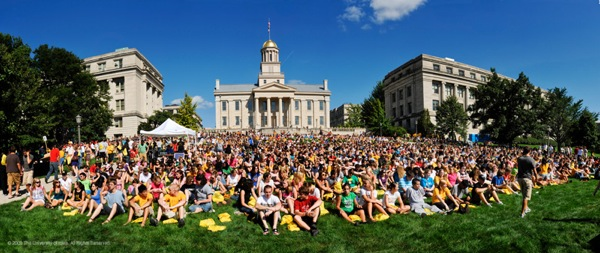
\includegraphics[width=0.6\columnwidth]{fig1}
    \label{fig:1}
\end{figure}

  \section{Neutrino Detection}

The detection of neutrinos is a crucial aspect of understanding nuclear reactions and the fundamental structure of matter.
The discovery of neutrino oscillations not only confirmed that neutrinos have mass but also opened up new avenues for research, such as the precise determination of the neutrino mass spectrum and the investigation of the potential for CP violation in the lepton sector.
Ongoing research aims to further understand their properties, including their masses, their role in the universe's matter-antimatter asymmetry, and potential new physics beyond the Standard Model.

In order to study them experimentally, we have to actually be able to detect them -- a task made complicated by the fact that neutrinos only interact with the weak force.
Trillions of neutrinos go through us humans every second and we don't notice because they don't really interact with us, instead passing right through.


\subsection{Types of Detectors}

Just as there are many ways to skin a cat, neutrinos can be detected using a number of detector technologies.
Each method harnesses different physical principles and technological advancements to observe these elusive particles.

Cherenkov detectors exploit the phenomenon of Cherenkov radiation, which occurs when a neutrino interacts with a medium at speeds greater than the speed of light in that medium.
This results in the emission of a faint blue light, which can be detected and analyzed.

The Super-Kamiokande detector in Japan uses a large tank filled with ultra-pure water.
It contains thousands of photomultiplier tubes that detect the Cherenkov radiation produced when neutrinos interact with the water.

Water Cherenkov detectors are a type of Cherenkov detector specifically utilizing water as the detection medium.
These detectors are characterized by their large volumes of water and arrays of photomultiplier tubes (PMTs) arranged around the tank.

The IceCube Neutrino Observatory at the South Pole uses a cubic-kilometer array of detectors embedded in the Antarctic ice, capturing Cherenkov radiation from high-energy neutrinos.

Scintillation detectors use materials that emit light when excited by the passage of a high-energy particle.
Neutrinos interact with a scintillator material, causing it to emit flashes of light, which are then detected by photodetectors.

The NOVA detector utilizes a liquid scintillator to detect neutrinos over long baselines, aiding in the study of neutrino oscillations.

Radio detectors capture the radio waves emitted by neutrino interactions in ice or other materials.
This method is particularly useful for very high-energy neutrinos.

The ANITA (Antarctic Impulse Transient Antenna) experiment detects high-energy neutrinos via the radio waves produced by neutrino interactions with the Antarctic ice.

Liquid Argon Time Projection Chambers (LArTPCs) use liquid argon as both the detector material and the medium for drift electrons generated by neutrino interactions.
The drifted electrons are then collected and analyzed to reconstruct the interaction.

The spatial resolution in LArTPCs depends on the drift length \( d \), drift field \( E \), and the electron mobility \( \mu \).

The DUNE (Deep Underground Neutrino Experiment) will use LArTPCs to study neutrino properties with high precision, particularly in the context of long-baseline neutrino oscillation experiments.



\subsection{Deep Underground Neutrino Experiment (DUNE)}

DUNE is a groundbreaking experiment designed to investigate neutrino properties by utilizing an innovative approach involving a large detector placed deep underground.
The primary goal of DUNE is to study neutrino oscillations
DUNE's experimental setup involves a neutrino beam generated from a high-intensity proton accelerator at Fermilab in Illinois.
The beam travels through the Earth to a massive detector located approximately 1,300 kilometers away, deep underground at the Sanford Underground Research Facility (SURF) in South Dakota.
The large scale of the detectors allows for the precise measurement of neutrino interactions, and its underground location minimizes interference from cosmic rays, thus improving the sensitivity of the experiment \cite{DUNE_Neut_Det}.

\begin{figure}[H]
  % https://www.dunescience.org/
  \centering
  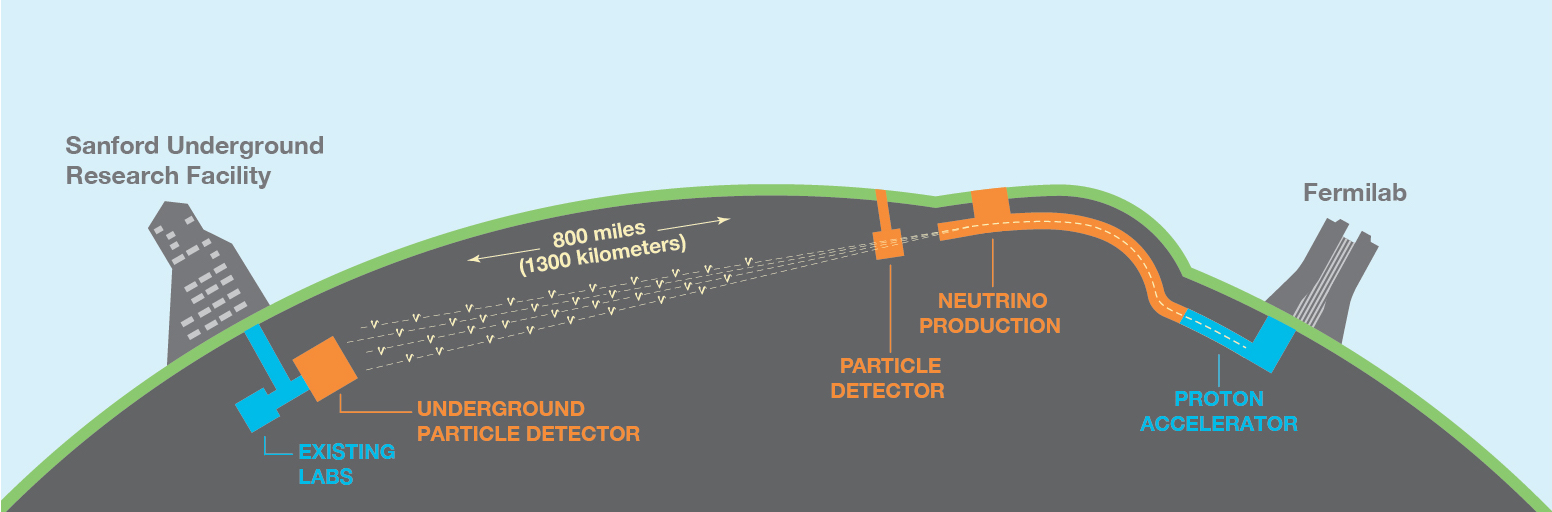
\includegraphics[width=120mm]{figures/dune.png}
  \caption{Cartoon of the DUNE setup \cite{DUNE_2020}}
  \label{dune}
\end{figure}

The plan is to have 2 sets of detectors, one at Fermilab, (near detector(ND)) and the other at SURF (far detector (FD)).
% https://arxiv.org/abs/2002.02967
The design of the DUNE far detector, grounded in cutting-edge Liquid Argon Time Projection Chamber (LArTPC) technology, is set to revolutionize particle physics.
This detector will be housed in a colossal volume of 70 kilotons of liquid argon, buried 1.5 kilometers underground \cite{DUNE_LBNF}.
To maximize the efficiency of physics experiments, the design splits this volume into four LArTPC modules, each with a usable "fiducial volume" of 10 kilotons, avoiding interactions near the edges.
To accommodate these massive detectors, approximately 800,000 tons of rock will be excavated, creating vast underground caverns.

The near detector will be built on the Argon cube concept.
The ND will have a modular design combined with a novel pixellated charge readout.
Previously, large detectors struggled with high demands for drift potentials and argon purity, which often led to risks of electric breakdown and purity losses.
By breaking down a large detector into smaller, independent modules, these risks are significantly reduced.
This modularity allows for easier maintenance and more reliable operation \cite{Biron_2020}.

\begin{figure}[H]
  % https://www.lhep.unibe.ch/research/detector_development/argoncube/index_eng.html
  \centering
  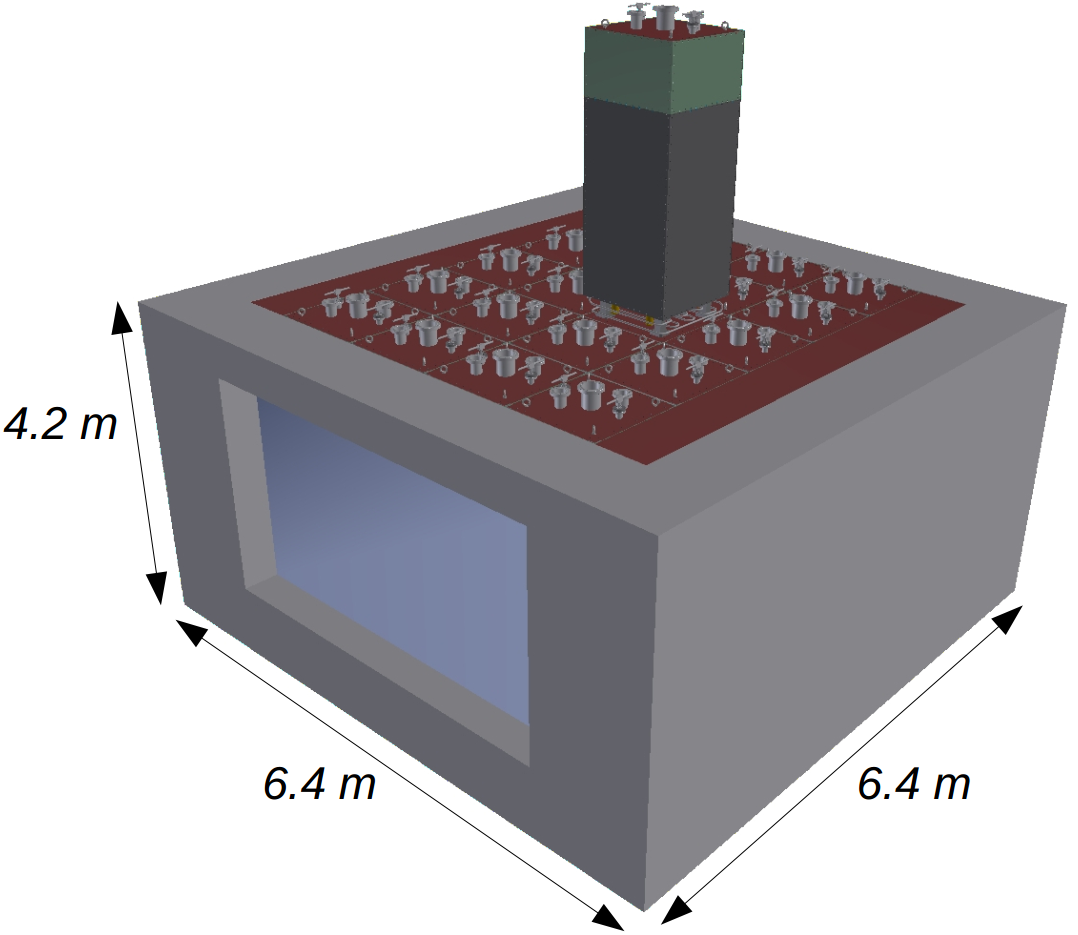
\includegraphics[width=80mm]{figures/nd.png}
  \caption{Design of the DUNE ND with $5 \times 7$ modules \cite{DUNE_2020a}}
  \label{nd}
\end{figure}

The fully pixelated charge readout adds another layer of sophistication, enabling precise event topology reconstruction.
This is important for handling high-multiplicity environments where pile-up could otherwise obscure important data.
Additionally, each module captures scintillation light to provide accurate timing information for neutrino events, further enhancing the detector's performance.

The real game-changer is the scalability of this design.
The modular approach means that the detector can be expanded to accommodate a very large active mass, opening up new possibilities for research and application.

\begin{figure}[H]
  % https://www.lhep.unibe.ch/research/detector_development/argoncube/index_eng.html
  \centering
  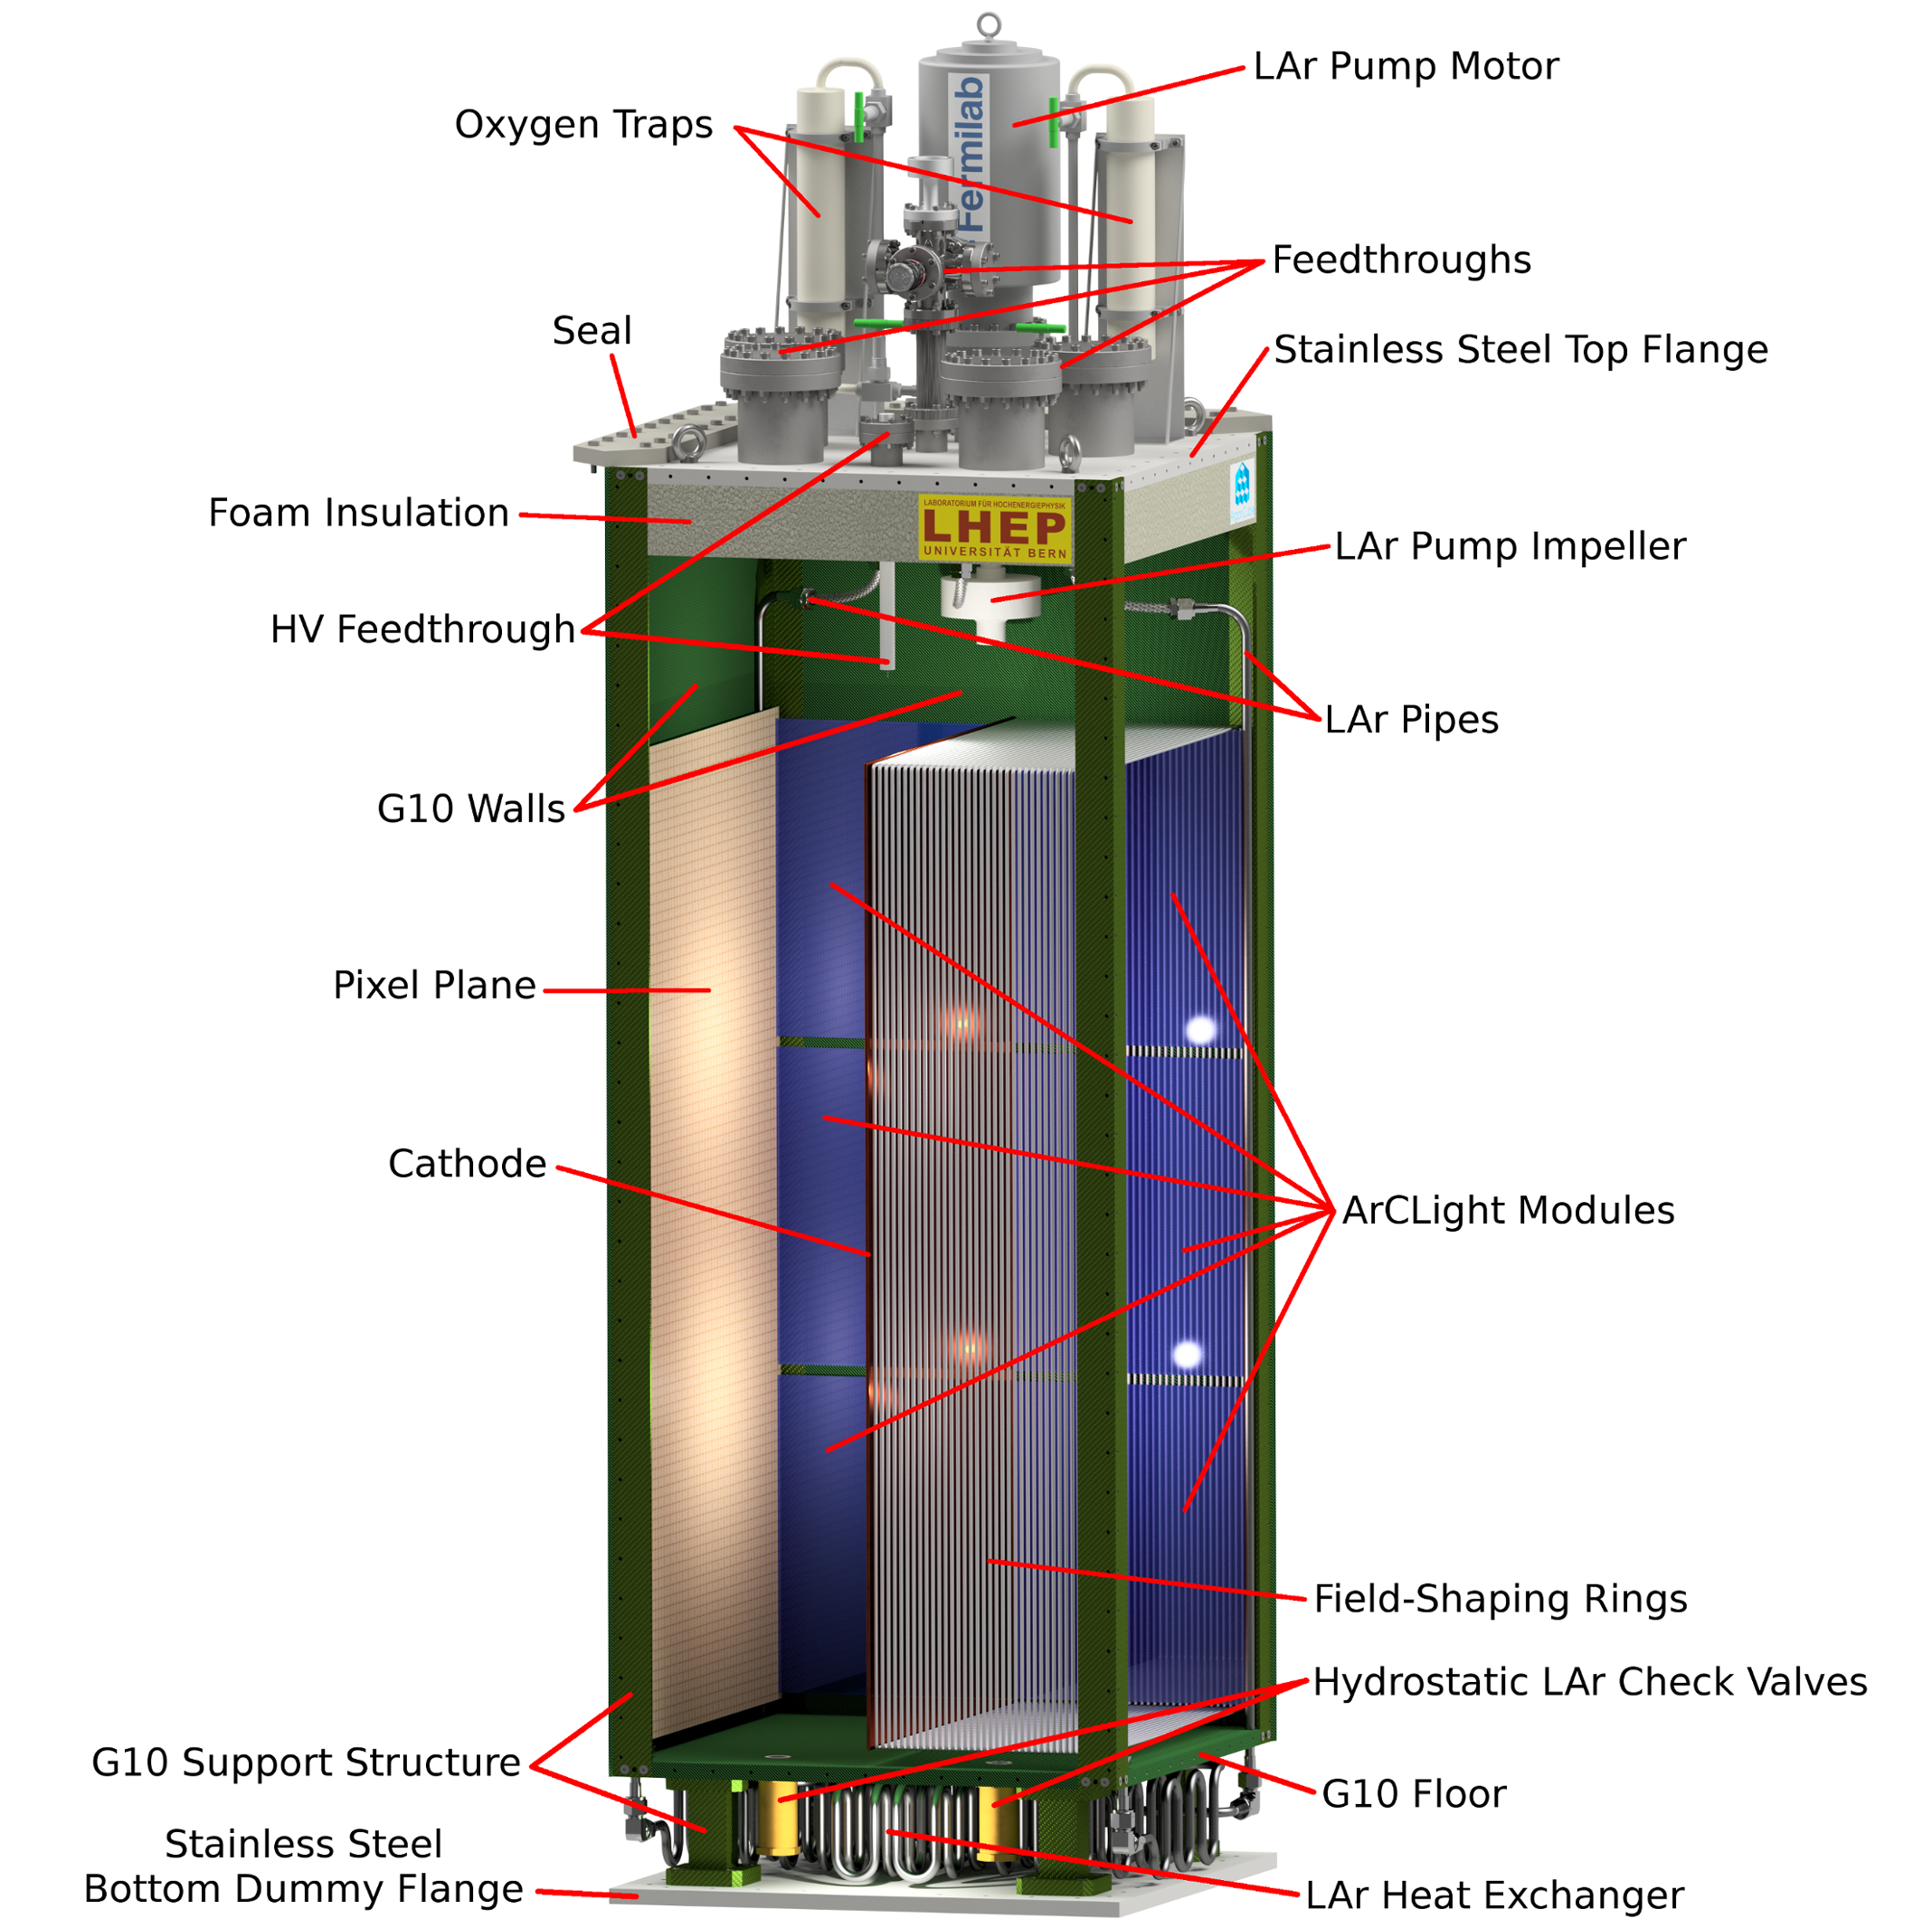
\includegraphics[width=80mm]{figures/ndModule.png}
  \caption{Cutaway image of a module\cite{DUNE_2020b}}
  \label{ndModule}
\end{figure}

Because of the novelty of the technology, a scaled down prototype  of the Argon cube detector called the $2 \times 2$ has been built.
Instead of having $5 \times7$ modules, it will have$2 \times 2$ modules.
Individual modules have already been built and tested before being put together to take data as part of a set.

\begin{figure}[H]
  % Original Image
  \centering
  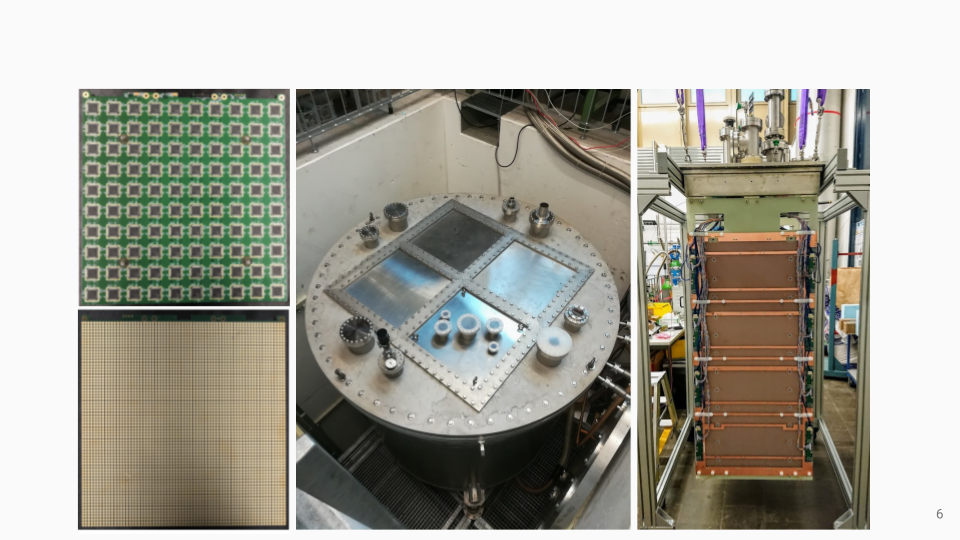
\includegraphics[width=120mm]{figures/ndPic.png}
  \caption{Pictures of the first module to be build (Module-0)}
  \label{ndPic}
\end{figure}

The scale of DUNE and its ambitious goals are reminiscent of the dramatic shifts in scientific paradigms brought about by the discovery of subatomic particles that challenged existing theories \cite{dune_tdr}.






  \section{Machine Learning}

When looking at artificial intelligence (AI), everything falls on a spectrum from easily explainable to being a black box when thinking about how the machine makes it's decisions.
On the easily explainable side of things, we have things like decision trees.

\begin{figure}[H]
  \centering
  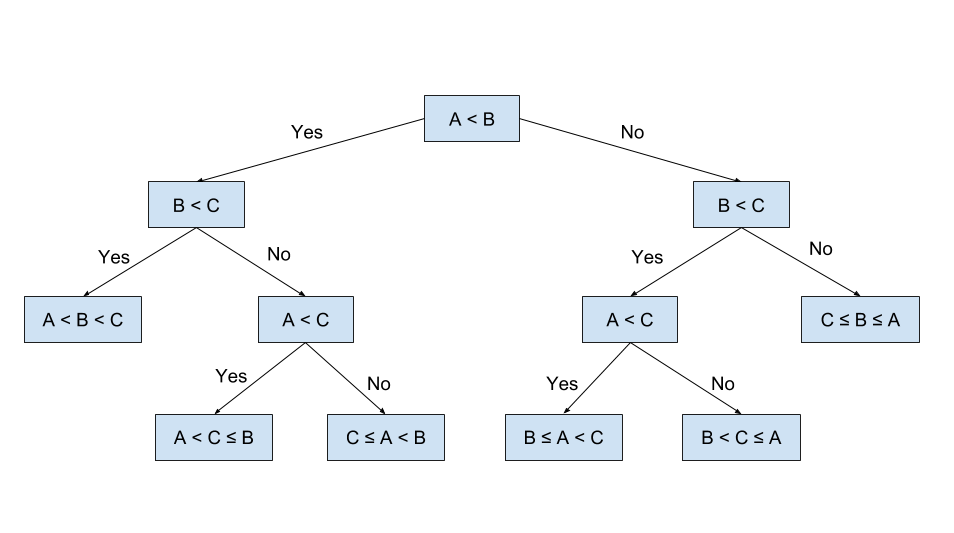
\includegraphics[width=120mm]{figures/decisionTree.png}
  \caption{Example of a basic decision tree}
  \label{decisionTree}
\end{figure}

A decision tree is where we sort the data by asking a sequence of questions and following the flowchart down to where it leads.
By the time we are at the bottom of the tree and have classified the data we can say exactly how the model does it's classification.
For instance if a decision tree is used for mortgage decisions and the model says no, we can query and learn that it said no because you had too low income or too low credit score for instance.

\begin{figure}[H]
  \centering
  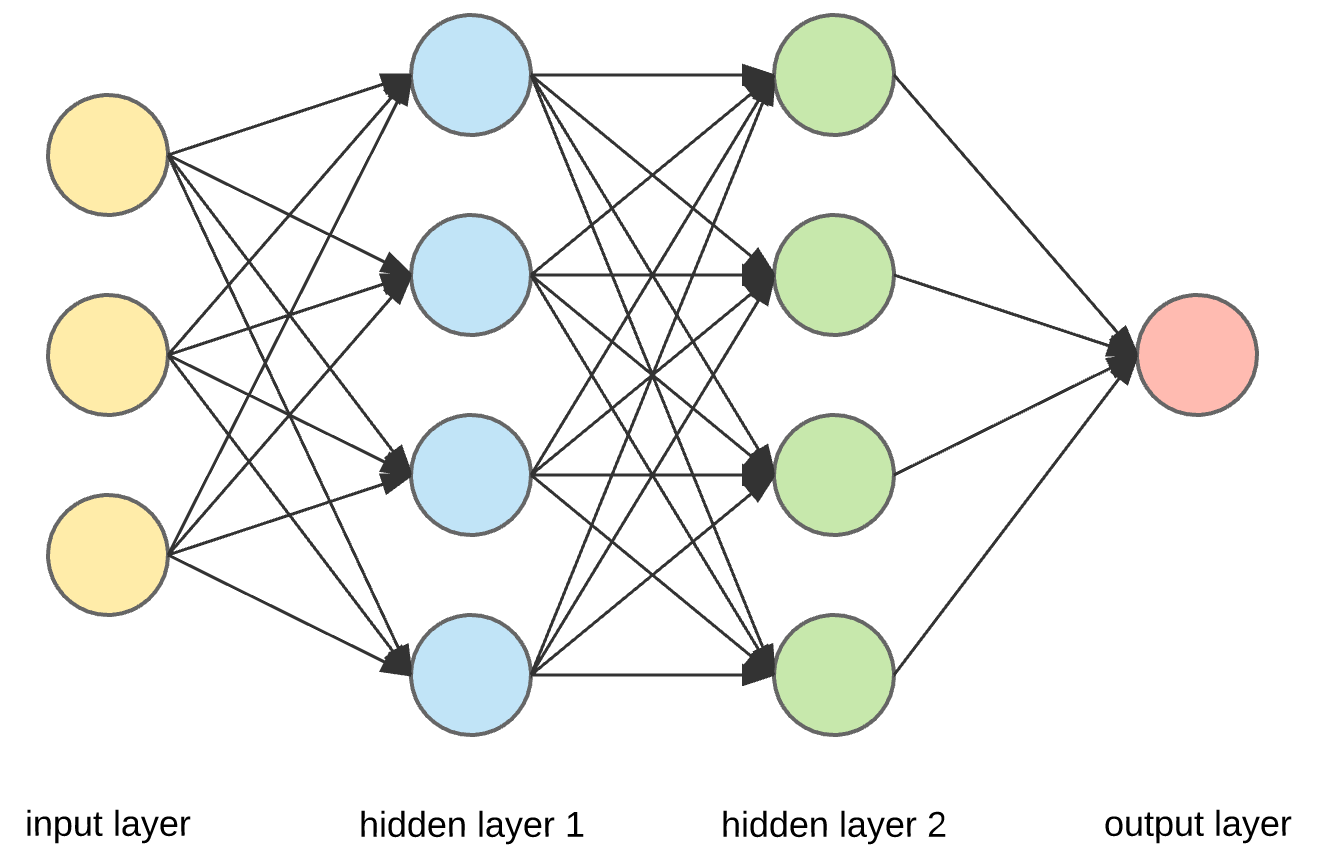
\includegraphics[width=120mm]{figures/neuralNet1.png}
  \caption{Example of a basic Neural Net}
  \label{neuralNet1}
\end{figure}

By contrast, a machine learning model like a neural net is almost a black box with regards to how the decisions are made.
We can query the model and ask it what it made its decisions based on, however, the features it picks out often isn't decipherable to humans in any way.
As in the previous example, if the answer to a mortgage is no, we have no real idea why the model made that decision.
That being said, neural networks are often able to come up with better outcomes for classification that simple models like decision trees are.
In the mortgage example, even if the neural net can't tell us how it comes to the conclusion of approving a loan, it is still more likely to be able to better tell who will be a good credit risk compared to the decision tree.
That's often the trade off that we make when deciding on a more opaque model.
That's why even though they are opaque in how they come up with their answers we still rely on them so heavily.
Because we can empirically test through monte-carlo studies how well they perform both in term of efficiency as well as how often these models misidentify the data that we are throwing at it.

While a neural network is opaque about how the decisions are made, the model itself doesn't have to be a black box for us.
We can take a peek under the hood and see how these models work.
To do so, we start up from the basic models like a perceptron and work our way to a graph neural network, finally connecting it to how neutrino reconstruction works.

\subsection{Perceptron Neuron}

A lot of things that seem incredibly easy to humans -- such as  recognizing the difference between say a cat and a dog -- are very difficult for computers to do.
What makes it difficult to make that sort of classification is that it is hard for humans to define concrete rules about what makes the picture of a cat different than the picture of a dog.
Neural nets approach this in a completely different fashion.

Instead of trying to define rules about the features that differentiate the picture of a dog vs a cat, we instead classify a whole bunch of pictures by hand.
\footnote{This is true only for supervised learning.
Unsupervised learning doesn't require classification by hand but have their own set of disadvantages}
Then throw those pictures at the algorithm with the correct answers and over time the computer learns to tell the difference between that of a dog and a cat.
We call an algorithm like this that separates things into two piles a binary classifier.
There are many different kinds of binary classifiers with a whole host of advantages and disadvantages but we will start with one that is simple to understand; the perceptron.

\begin{figure}[H]
  \centering
  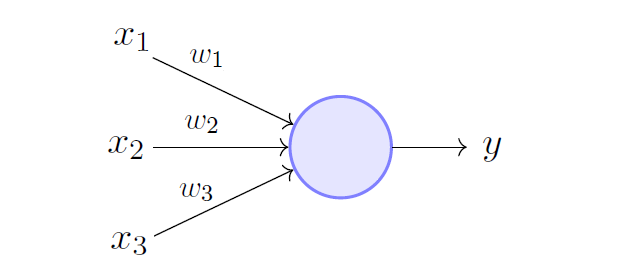
\includegraphics[width=120mm]{figures/perceptron1.png}
  \caption{Perceptron Neuron \cite{El-Amir_Hamdy_2019}}
  \label{perceptron1}
\end{figure}

A perceptron takes a number of inputs that are binary in nature and produce a single binary output \cite{Freund_Schapire_1998} ie.is this a dog? The figure \ref{perceptron1} has 3 inputs ($x_1$, $x_2$ and $x_3$) although, more or fewer inputs may be used.
Each input then is given a weight -- $w_1$, $w_2$ and $w_3$ in this case -- and the output calculated thus.

\begin{align}
  y = \begin{cases}
    0 \textrm{ if } \sum_i w_i x_i \leq \textrm{threshhold},\\
    1 \textrm{ if } \sum_i w_i x_i > \textrm{threshhold},\\
  \end{cases}
\end{align}

Used in this fashion, a perceptron can only make simple choices.
Raising the threshold makes the classification tighter while lowering it loosens the classification.
Because the output of a perceptron is binary, for more subtle distinctions, we can use the output of a perceptron to feed into the input of the next one thus creating a network that is more able to measure subtlety.

\begin{figure}[H]
  \centering
  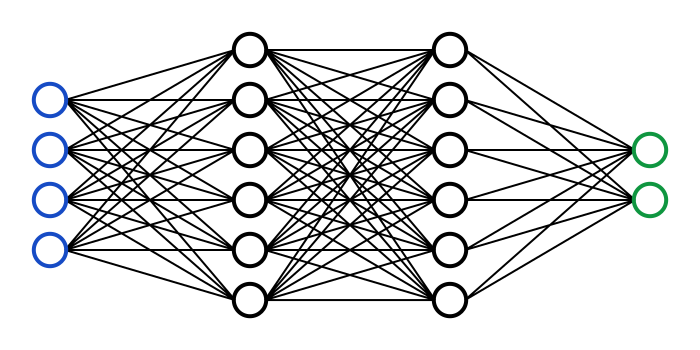
\includegraphics[width=120mm]{figures/network.png}
  \caption{Perceptron network \cite{Zhou_2020}}
  \label{network}
\end{figure}

Varying the weights of the inputs in combination with the threshold for the output allows us to get different models of classification.
The neurons in the first layer are only able to make simple decisions based on the raw input but because we use their output as the input to the second layer, the second layer can make more abstract decisions with a degree of subtlety impossible not only with one perceptron but also with even a single layer of perceptrons.
The complexity of the discrimination by the classifier increasing with both the number and layers of perceptrons in the network.

With the correct weights and threshold values, we can get any binary classifier we want using a set of perceptrons.
That, however, puts us back at our original problem of classifying whether something is a dog; namely, if we knew what features to look for (i.e.\ what weights and threshold to use) it wouldn't be hard explaining to a computer what a dog was.
The true innovation comes with using learning algorithms that don't require input from the programmer to set these weights and thresholds.

  If we want to use algorithms that can adjust weights and thresholds (otherwise called biases) automatically, we need some method where a small change in the weight only causes a small change in the output.
Because perceptrons are binary, this is impossible to do with only perceptrons.

  A small change in the weight to an input to the perceptron can flip the output entirely.
While this small change in weight can make one of the outputs of the network better, it may also affect the rest of the network behave in unpredictable ways.
Going back to the dog and cat example, while changing the weight slightly may make it better at recognizing dogs, it may wreak havoc on how cats are identified.

  This is where sigmoid neurons come in.

\subsection{Sigmoid Neuron}

While perceptrons are effectively step functions, flipping from $0$ to $1$, sigmoids are more smoothed out.
This means that a small change in the weight can lead to a small change in output\cite{Nielson_2020}.
The sigmoid function can be written as

\begin{align}
  \sigma = \frac{1}{1 + e^{-z}}
\end{align}

This means that a sigmoid neuron can be written as

\begin{align}
  \frac{1}{1 + e^{-\sum_i w_i x_i - b}}
\end{align}

where the $b$ stands for the bias of every input.
While this looks different than the perceptron at first glance it is just a more smoothed out version of it.
One key thing that we lose with the introduction of sigmoids is the linearity that perceptrons afforded us.
What we gain is the ability for our programs to automatically adjust their weights and biases because a small change in weights does lead to small change in output as shown in equation \ref{bias}.

\begin{align}\label{bias}
  \Delta y \approx \sum_i \frac{\partial y}{\partial w_i}\Delta w_i + \frac{\partial y}{\partial b}\Delta b
\end{align}

\begin{figure}[H]
  % https://blog.roboflow.com/activation-function-computer-vision/
  \centering
  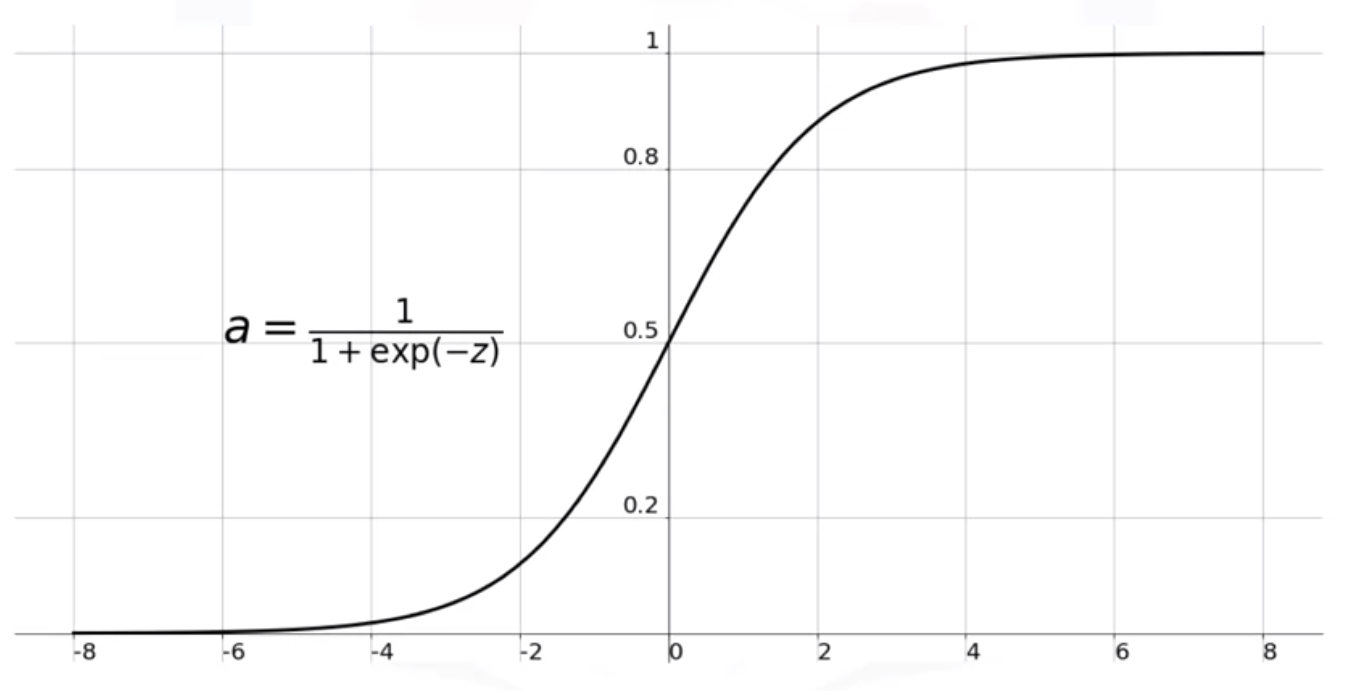
\includegraphics[width=80mm]{figures/sigmoid.png}
  \caption{Sigmoid Function \cite{Potrimba_2023}}
  \label{network}
\end{figure}

More than the exact formula of the sigmoid neuron what matters is the shape.
As a result, other neurons can be used in its stead which retain the property of having a small change in weight lead to a small change in output.
Some of the more popular of these functions (called activation functions) are RELU and softmax.
Each have their own advantages and disadvantages and may even be mixed in the same neural network


 

  % \section{heading 1: my chapter 1}

Heading 1 is the style you should use for the following headings in your thesis: List of Tables, List of Figures (List of Abbreviations, Schemes, and so on), Chapter titles, References, and Appendix titles. If you are writing in APA style, note that the titles formatted as Heading 1 do not count as an APA heading.  

I want to cite something here \parencite{zuo2019standing}. I want to want to try cite~\textcite{zuo2019standing} with in-line style.

\subsection{heading 2: Use for Your broadest Subheading Level, Centered, Bold, Title Case}

Heading 2 is the first major subheading style. If you are writing in APA style, this heading corresponds to a Level 1 APA heading.  

\subsubsection{heading 3: Use for Your Next Heading Level, Left-aligned, Bold, Title Case}

Heading 3 is the second major subheading style. If you are writing in APA style, this heading corresponds to a Level 2 APA heading. 

\paragraph{Heading 4: This Heading is Left-aligned, Boldface Italics, Title Case}
This is an additional heading level, should your thesis require this level of specificity.

Let me add a figure here~\cref{fig:1}:
\begin{figure}[h]
    \centering
    \captionsetup{width=0.6\linewidth} %% change width to adjust the caption alignment
    \caption{Old capital museum}
    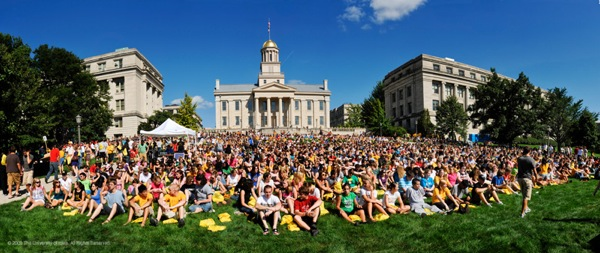
\includegraphics[width=0.6\columnwidth]{fig1}
    \label{fig:1}
\end{figure}

  % \section{my chapter 2}

Lorem ipsum dolor sit amet, consectetuer adipiscing elit.  Ut purus elit, vestibulum ut, placeratac,  adipiscing vitae,  felis.   Curabitur dictum gravida mauris.  

Nam arcu libero,  nonummy eget,consectetuer id, vulputate a, magna. Donec vehicula augue eu neque. Pellentesque habitant morbitristique senectus et netus et malesuada fames ac turpis egestas. Mauris ut leo. Cras viverra metusrhoncus sem.  Nulla et lectus vestibulum urna fringilla ultrices. 

I want to cite something here \parencite{fennell2018predicting}. I want to want to try cite~\textcite{zuo2019standing} with in-line style.
Add this table here:

\begin{table}[ht]
    \centering
    \captionsetup{width=0.8\linewidth} %% change width to adjust the caption alignment
    \caption{Sample table}
    \begin{tabular}{cccccc}
         \hline
         \textbf{Column 1} & \textbf{Column}  & \textbf{Column 3} & \textbf{Column 4} & \textbf{Column 5} & \textbf{Column 6}\\
         \hline
         \textbf{Row 1} & 12.34 & 12.34 & 12.34 & 12.34 & 12.34 \\
         \hline
         \textbf{Row 2} & 12.34 & 12.34 & 12.34 & 12.34 & 12.34 \\
         \hline
    \end{tabular}
    \label{table:table1}
\end{table}

Lorem ipsum dolor sit amet, consectetuer adipiscing elit.  Ut purus elit, vestibulum ut, placeratac,  adipiscing vitae,  felis.   Curabitur dictum gravida mauris.  
Nam arcu libero,  nonummy eget,consectetuer id, vulputate a, magna. Donec vehicula augue eu neque. Pellentesque habitant morbitristique senectus et netus et malesuada fames ac turpis egestas. Mauris ut leo. Cras viverra metusrhoncus sem.  Nulla et lectus vestibulum urna fringilla ultrices~\cref{table:table1}. 


  % \section{my chapter 3}

Lorem ipsum dolor sit amet, consectetuer adipiscing elit.  Ut purus elit, vestibulum ut, placeratac,  adipiscing vitae,  felis.   Curabitur dictum gravida mauris.  

Nam arcu libero,  nonummy eget,consectetuer id, vulputate a, magna. Donec vehicula augue eu neque. Pellentesque habitant morbitristique senectus et netus et malesuada fames ac turpis egestas. Mauris ut leo. Cras viverra metusrhoncus sem.  Nulla et lectus vestibulum urna fringilla ultrices. \textcite{zuo2017state}

Lorem ipsum dolor sit amet, consectetuer adipiscing elit.  Ut purus elit, vestibulum ut, placeratac,  adipiscing vitae,  felis.   Curabitur dictum gravida mauris.  
Nam arcu libero,  nonummy eget,consectetuer id, vulputate a, magna. Donec vehicula augue eu neque. Pellentesque habitant morbitristique senectus et netus et malesuada fames ac turpis egestas. Mauris ut leo. Cras viverra metusrhoncus sem.  Nulla et lectus vestibulum urna fringilla ultrices. 

Let me add another figure here:

\begin{figure}[h]
    \centering
    \captionsetup{width=0.7\linewidth} %% change width to adjust the caption alignment
    \caption{Kinnick stadium}
    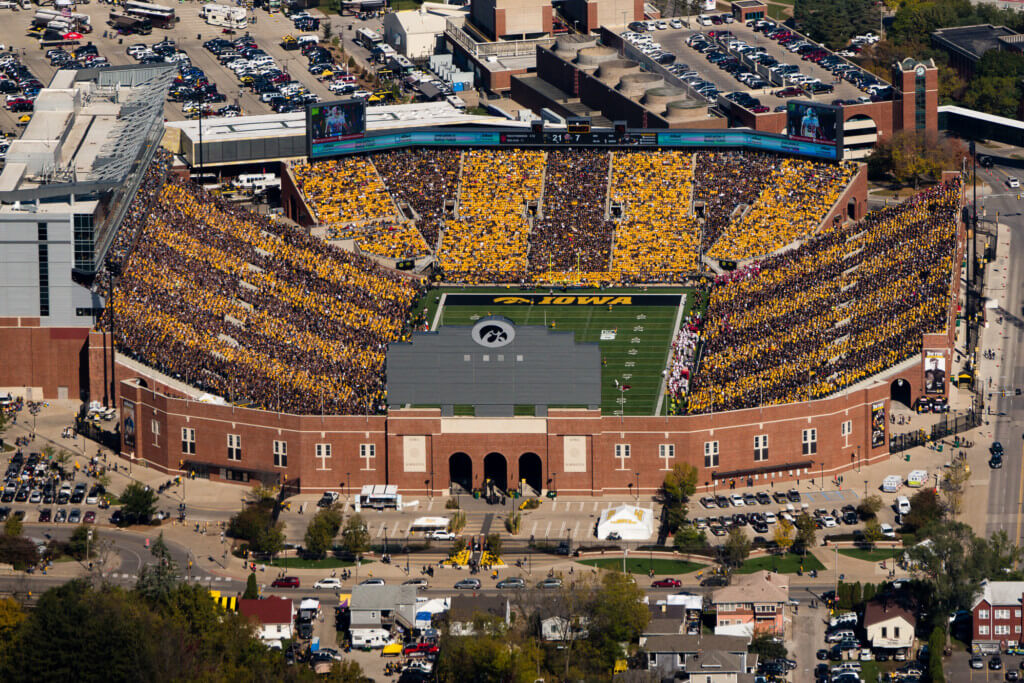
\includegraphics[width=0.7\columnwidth]{fig2}
    \label{fig:2}
\end{figure}

\subsection{heading 2: Use for Your broadest Subheading Level, Centered, Bold, Title Case}

Lorem ipsum dolor sit amet, consectetuer adipiscing elit.  Ut purus elit, vestibulum ut, placeratac,  adipiscing vitae,  felis.   Curabitur dictum gravida mauris~(\cref{fig:2}).  
Nam arcu libero,  nonummy eget,consectetuer id, vulputate a, magna. Donec vehicula augue eu neque. Pellentesque habitant morbitristique senectus et netus et malesuada fames ac turpis egestas. Mauris ut leo. Cras viverra metusrhoncus sem.  Nulla et lectus vestibulum urna fringilla ultrices. 

  %% main contents %%

  %% ref bibtex%%
  \clearpage

  \bibliographystyle{unsrt}
  \bibliography{ref.bib}
  \nocite{*}
  %% ref bibtex%%

  %% appendix %%
  % \appendix
  % \newcommand{\hbAppendixPrefix}{A}
\renewcommand{\thefigure}{\hbAppendixPrefix.\arabic{figure}}
\setcounter{figure}{0}
\renewcommand{\thetable}{\hbAppendixPrefix.\arabic{table}} 
\setcounter{table}{0}

\let\svaddcontentsline\addcontentsline
\renewcommand\addcontentsline[3]{%
      \ifthenelse{\equal{#1}{lof}}{}%
        {\ifthenelse{\equal{#1}{lot}}{}{\svaddcontentsline{#1}{#2}{#3}}}}

\section{APPENDIX \hbAppendixPrefix: Numeric data}

The Appendix (A, B, and so on) heading is formatted as a Heading 1. Note that if you include only one Appendix, you do not need to assign it a letter. 

Make a table in Appendix A:
\begin{table}[ht]
    \centering
    \captionsetup{width=0.8\linewidth} %% change width to adjust the caption alignment
    \caption{Sample table}
    \begin{tabular}{cccccc}
         \hline
         \textbf{Column 1} & \textbf{Column}  & \textbf{Column 3} & \textbf{Column 4} & \textbf{Column 5} & \textbf{Column 6}\\
         \hline
         \textbf{Row 1} & 12.34 & 12.34 & 12.34 & 12.34 & 12.34 \\
         \hline
         \textbf{Row 2} & 12.34 & 12.34 & 12.34 & 12.34 & 12.34 \\
         \hline
    \end{tabular}
    \label{table:tableA1}
\end{table}

And I am going to ref this table~\cref{table:tableA1}.
Lorem ipsum dolor sit amet, consectetuer adipiscing elit.  Ut purus elit, vestibulum ut, placeratac,  adipiscing vitae,  felis.   Curabitur dictum gravida mauris.  
Lorem ipsum dolor sit amet, consectetuer adipiscing elit.  Ut purus elit, vestibulum ut, placeratac,  adipiscing vitae,  felis.   Curabitur dictum gravida mauris.  
Lorem ipsum dolor sit amet, consectetuer adipiscing elit.  Ut purus elit, vestibulum ut, placeratac,  adipiscing vitae,  felis.   Curabitur dictum gravida mauris.  
Lorem ipsum dolor sit amet, consectetuer adipiscing elit.  Ut purus elit, vestibulum ut, placeratac,  adipiscing vitae,  felis.   Curabitur dictum gravida mauris.  
Lorem ipsum dolor sit amet, consectetuer adipiscing elit.  Ut purus elit, vestibulum ut, placeratac,  adipiscing vitae,  felis.   Curabitur dictum gravida mauris.  

  % \renewcommand{\hbAppendixPrefix}{B}
\renewcommand{\thefigure}{\hbAppendixPrefix.\arabic{figure}}
\setcounter{figure}{0}
\renewcommand{\thetable}{\hbAppendixPrefix.\arabic{table}} 
\setcounter{table}{0}

\section{APPENDIX \hbAppendixPrefix: Image data}

Lorem ipsum dolor sit amet, consectetuer adipiscing elit.  Ut purus elit, vestibulum ut, placeratac,  adipiscing vitae,  felis.   Curabitur dictum gravida mauris.
Let me add a figure here~\cref{fig:B1}:

\begin{figure}[h]
    \centering
    \captionsetup{width=0.7\linewidth} %% change width to adjust the caption alignment
    \caption{Old capital museum}
    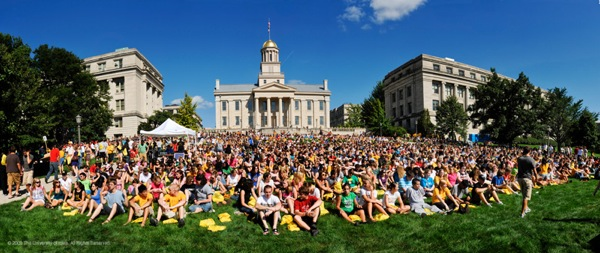
\includegraphics[width=0.7\columnwidth]{fig1}
    \label{fig:B1}
\end{figure}


  %% appendix %%


\end{doublespace}


\end{document}
